\documentclass[12pt]{report}
\usepackage{amssymb}
\usepackage{amsmath}

\usepackage{multicol}
\usepackage{graphicx}
\usepackage{subfigure}
\usepackage{verbatim}

%\usepackage{adjustbox}

\usepackage[letterpaper,left=1cm,right=2cm, top=1.5cm,
bottom=1.5cm,head=0cm,foot=1cm]{geometry}

\parindent=0in


\newcommand{\m}{\mbox{m }}
\newcommand{\kg}{\mbox{kg}}
\newcommand{\s}{\mbox{s}}
\newcommand{\ke}{\mbox{\small KE}}
\newcommand{\pe}{\mbox{\small PE}}
\newcommand{\un}{\mbox{ u}}


\newcommand{ \probDir}[1]{{ \bf\small #1 \mbox{  }}}

\newcommand{ \breakList}{\setcounter{saveenum}{\value{enumi}} \end{enumerate}}
\newcommand{ \contList}{\begin{enumerate} \setcounter{enumi}{\value{saveenum}}}

\newcounter{saveenum}

\def \wspace{5cm}

%%%%%%%%%%%%%%%%%%%%%%%%%%%%%%%%%%%%%%%%%
\begin{document}

{\bf{Honors Physics} \hfill Notepage: Friction \hfill {Mr. Kelley}} \\ \\
%%%%%%%%%%

\vspace{1cm}

\hfill \parbox{12cm}{In order to know the force of friction we must understand the normal force acting on an object.  The normal force is the force that ``pushes back" on an object resting on a surface.  $F_\bot$ can be thought of as how hard the two surfaces are pushing together. \\ \\ It makes sense, then, that the greater the normal force, the greater the force of friction will be.  In fact, the force of friction is proportional to the normal force.  This equation reflects that:} \hspace{4cm}
$$ F_f = \mu F_\bot$$

\vspace{.75cm}

\hfill \parbox{14cm}{Consider a mass $m=14 \mbox{ }\kg$, and a force $F_1 = 100$ N pulling it horizontally along a surface.  If the coefficient of friction is $\mu = .66$, what will the resulting acceleration of the object be?} \hspace{3cm}

\vspace{.75cm}

\hfill 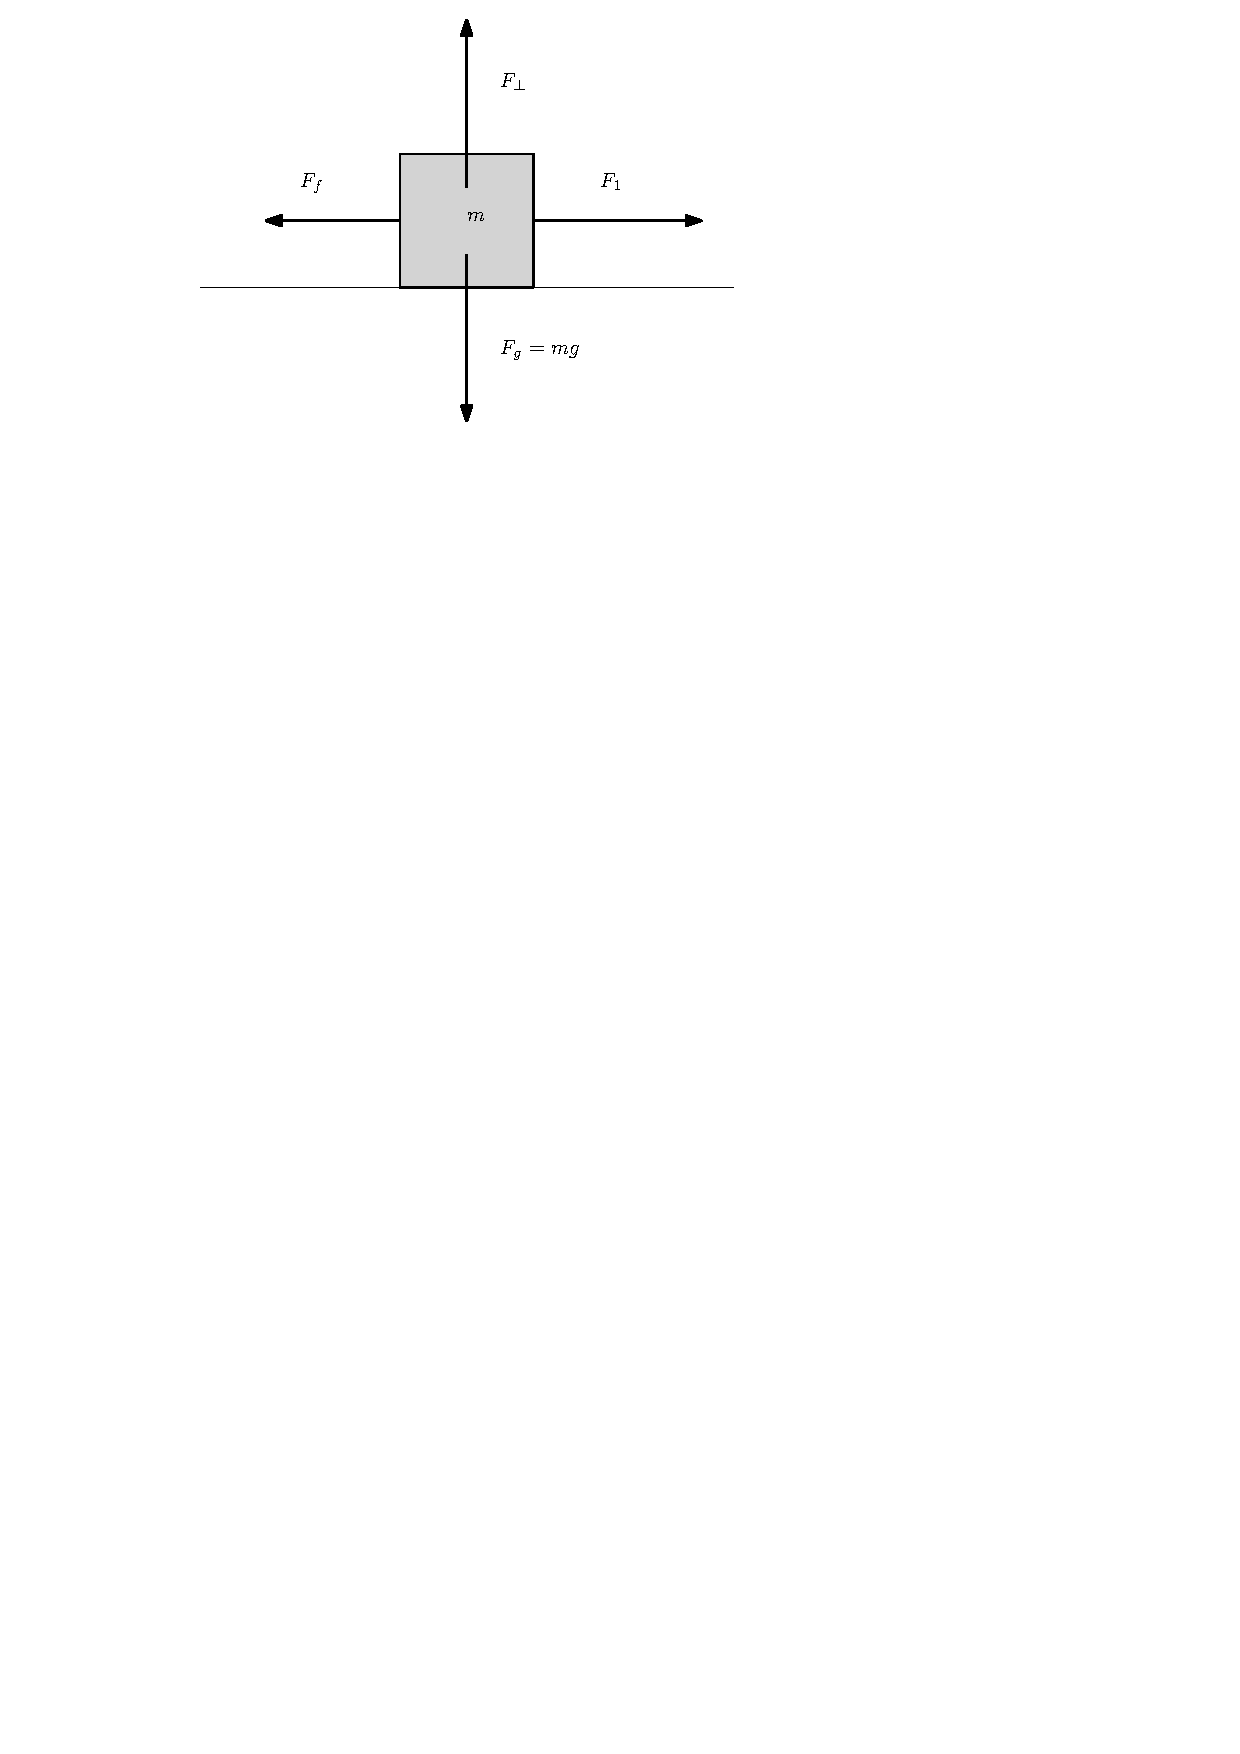
\includegraphics{box1} \hfill \mbox{}

\vspace{1cm}

\hspace{2cm} \parbox{6cm}{$\sum F_y = 0$, since there is no acceleration in the $y$-direction.  That also tells us that $F_\bot = mg$. (Why?)} \hfill \parbox{6cm}{In the $x$-direction we have $\sum F_x = F_1 - F_f$.  The negative sign is because \emph{friction always resists motion}.  We then have $\sum F_x = F_1 - \mu F_\bot=ma$ (Remember $\sum F$ is always equal to $ma$.  See Newton's 2$^{\mbox{\tiny nd}}$ Notepage)} \hspace{2cm}

\vfill

\hfill Continue the problem to solve for $a$ \hfill [Ans: $a = 0.675 \m/\s^2$] \hfill \mbox{}

\end{document}